\begin{frame}{Example finding a path between A and B with a network}
	\centering
	\only<1>{
		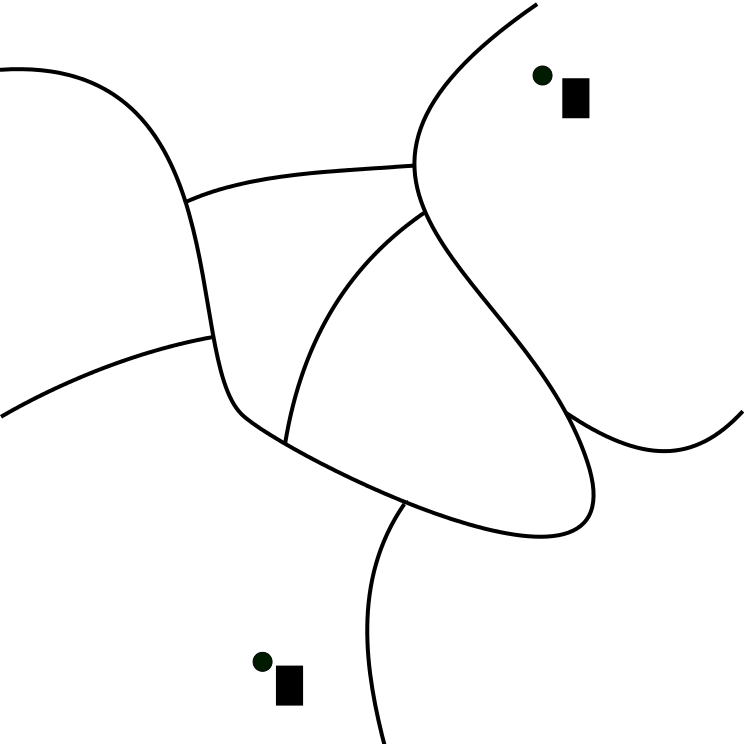
\includegraphics[width=0.6\textwidth]{net-example1.png}
	}
	\only<2>{
		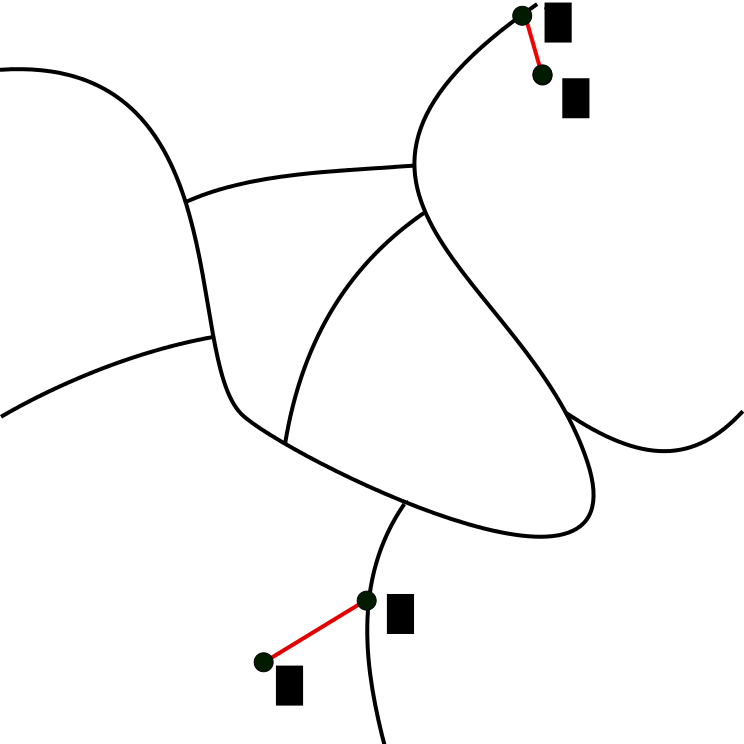
\includegraphics[width=0.6\textwidth]{net-example2.png}
	}
	\only<3>{
		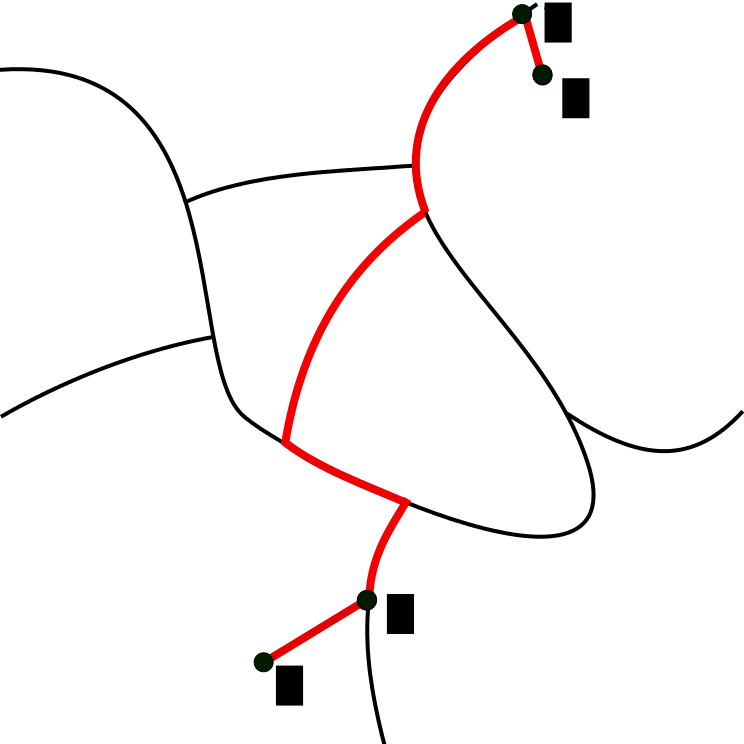
\includegraphics[width=0.6\textwidth]{net-example3.png}
	}
\end{frame}

\begin{frame}{Building the network}
	\begin{itemize}
		\item Chosing how to build the network is really important 
		\item Well chosen network results in high-quality paths
		\item Paths can become really expensive if the network is not well chosen. 
		\item To dense networks result in high computing time for $\overline{A}, \overline{B}$
		\item A network that is to sparse result in high computing time for $B$, $\overline{B}$
	\end{itemize}
	
	\note{
		A network is well chosenwhen it closely aligns with the lowest-cost subpaths over the terrain.
	}
\end{frame}
